\section{Lecture Ten: Bending of Beams}
\begin{itemize}
    \item Plane sections refer to vertical lines which are perpendicular to the length of a member. After the member is bent, these vertical lines rotate but otherwise remain straight.
    \begin{center}
        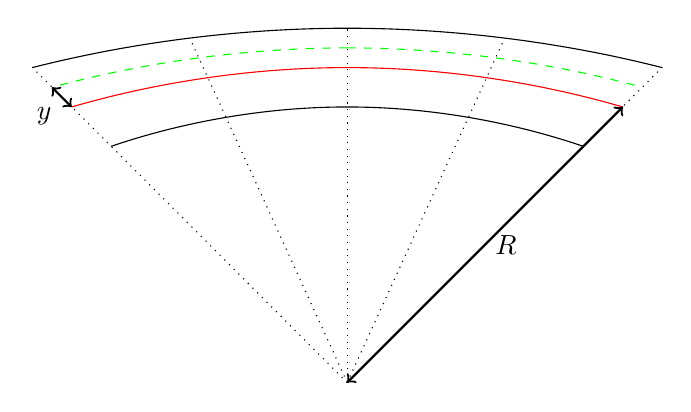
\begin{tikzpicture}
            \coordinate (O) at (0,0);
            \coordinate (A) at (-4, 4);
            \coordinate (A') at (-3, 3);
            \coordinate (B) at (4, 4);
            \coordinate (B') at (3, 3);
            \coordinate (A'') at (-3.5, 3.5);
            \coordinate (B'') at (3.5, 3.5);
            \coordinate (A''') at (-3.75, 3.75);
            \coordinate (B''') at (3.75, 3.75);
        
            \draw[] (0,4.5) parabola (A);
            \draw[] (0,4.5) parabola (B);
            \draw[] (0,3.5) parabola (A');
            \draw[] (0,3.5) parabola (B');
            \draw[color=red] (0,4) parabola (A'');
            \draw[color=red] (0,4) parabola (B'');
            \draw[dashed, color=green] (0,4.25) parabola (A''');
            \draw[dashed, color=green] (0,4.25) parabola (B''');            
            \foreach \x in {-4,-2,...,4}{
                \draw[dotted] (O) -- (\x,-0.031*\x*\x+4.5);
            }
            \draw[<->,thick] (O) -- (B'') node[midway, right] {$R$};
            \draw[<->,thick] (A'') -- (A''') node[midway, below left] {$y$};

        \end{tikzpicture}
    \end{center}
    We can divide up the plane sections such that they subtend an angle of $\phi$ and the length of the red line (neutral section) they subtend is of unit length. As a result:
    \begin{equation}
        \phi = \frac{1}{R}
        \label{eq:}
    \end{equation}
    where $R$ is the radius. Lengths above the red mark get stretched while lengths below the red mark gets shrunk. If we take a section $y$ above the neutral length, it gets deformed a length:
    \begin{equation}
        L_\text{def} = \phi (R+y) = \phi R+\phi y
        \label{eq:}
    \end{equation}
    and the strain would be given by:
    \begin{equation}
        \epsilon = \frac{L_\text{def}-L_0}{L_0}=\frac{\phi R+\phi y-1}{1} = \phi y
        \label{eq:}
    \end{equation}
    As a result, the stress increases linearly:
    \begin{equation}
        \sigma_y = E\phi y
        \label{eq:}
    \end{equation}
    \item If we integrate the stresses in the $y$ direction, then we get:
    \begin{equation}
        N=\int_A \sigma_y dA = E\phi \int_A y dA
        \label{eq:}
    \end{equation}
    We can calculate the curvature as:
    \begin{equation}
        \phi = \frac{M}{EI}
        \label{eq:}
    \end{equation}
    so
    \begin{equation}
        \sigma_y = \frac{My}{I}.
        \label{eq:}
    \end{equation}
    which is referred as \textbf{Navier's equation.}
    \item The moment can be calculated by:
    \begin{equation}
        M = \int_A \sigma_y y dA = E\phi \int_A y^2 dA = E\phi I
        \label{eq:}
    \end{equation}
    where $I$ here is the second moment of inertia: which is the moment of inertia divided by density.
    \item The moment of inertia of a beam is:
    \begin{equation}
        I = \frac{1}{12}bh^3
        \label{eq:}
    \end{equation}
    
\end{itemize}